% !TeX root = master.tex

\section{Cálculo de variaciones}

\subsection{Herramientas previas y repaso}

Necesitaremos recordar algunas nociones y teoremas básicos sobre derivabilidad:

\begin{definition}
\label{funciondiferenciable}

Sea $\funcion{f}{X}{Y}$ con $X,Y$ espacios normados. Se dice que $f$ es \textbf{diferenciable} en un punto $a\in\overset{\circ}{A}$, si existe una aplicación lineal continua $\funcion{T}{X}{Y}$ verifiando:

\[
\limite{x}{a}{\frac{\norm{f(x)-f(a)-T(x-a)}}{\norm{x-a}}} = 0
\]

$T$ se denota por $Df(a)$ y se llama \textit{diferencial de $f$}.
\end{definition}

\begin{theorem}[derivada de una integral respecto de un parámetro]
\label{derivadaparametro}
Sea $X\subset\R^n$ y $(X,\mathcal{A},\mu)$ un espacio medible, $I$ un intervalo cerrado y sea $\funcion{f}{I\times X}{\R}$ tal que:

\begin{enumerate}[(a)]
\item $\forall t \in I$, $x\mapsto f(t,x)$ es integrable.
\item $\forall x\in X$, la función $t\mapsto f(t,x)$ es derivable en $t\in I$.
\item Existe $\funcion{g}{X}{\R}$ integrable tal que

\[
\left|\derivada{f}{t}(t,x)\right|\leq |g(x)| \espacio \forall x\in X\; \forall t \in I
\]

Entonces la función $F(t)=\int_Xf(t,x)dx$ es derivable en $t_0$ y la derivada es 
\[
F'(t_0)=\displaystyle\int_X\derivada{f}{t}(t_0,x)dx
\]
\end{enumerate}

\end{theorem}

\subsection{Problema general del cálculo de variaciones}

Primeramente definimos un tipo de funciones llamadas \textit{funciones test} o \textit{funciones de la clase de Schwartz}, junto con algunos resultados que usaremos bastante para trabajar con ellas.

\begin{definition}
\label{funcionestest}
Dado $I$ intervalo, se llama \textit{espacio de funciones test} al conjunto:

\[
\mathcal{D} = \{\phi\in C^{\infty}(a,b): \; \exists J\subset(a,b) \text{ compacto: } \phi(x)=0 \text{ si } x \in J\}
\]
\end{definition}

\begin{lemma}
\label{existanciaphi}
Dado $x_0\in(a,b)$ y $\varepsilon>0$ tal que $[x_0-\varepsilon, x_0+\varepsilon]\subset(a,b)$, existe $\phi\in\mathcal{D}(a,b)$ tal que $\phi(x)>0$ si $x\in(x_0-\varepsilon,x_0+\varepsilon)$ y $\phi(x)=0$ en otro caso.
\end{lemma}

\begin{proof}
La demostración la vamos a hacer por construcción. Sea $\funcion{g}{\R}{\R}$ definida por:

\[
g(x)=\left\{
\begin{array}{cc}
e^{1/x} & x<0 \\
0 & x\geq 0

\end{array}
\right.
\]

Tenemos que $\limite{x}{0^-}{g(x)}=0$, luego $g$ es continua. Veamos que de hecho $g\in C^{\infty}$. Su derivada es:

\[
g'(x)=\left\{
\begin{array}{cc}
e^{1/x}\left(-\frac{1}{x^2}\right) & x<0 \\
0 & x> 0

\end{array}
\right.
\]

Mediante un proceso iterativo llegamos a:

\[
g^{n)}(x)=\left\{
\begin{array}{cc}
e^{1/x}\frac{R(x)}{x^{2n}} & x<0 \\
0 & x> 0

\end{array}
\right.
\]

donde $R(x)$ es un cierto polinomio que no nos interesa calcular. Queremos ver que $\limite{x}{0^-}{g^{n)}(x)}=0$. Haciendo el cambio $y=-\frac{1}{x}$, el anterior límite equivale a 
\[
\limite{y}{+\infty}{\frac{y^{2n}}{e^y}}=0 \Longrightarrow g\in C^{\infty}
\]

Con lo anterior, solo nos queda definir la función buscada de forma que sea una función test, es decir, la definimos como:

\[
\phi(x)=g(x-(x_0+\varepsilon))g((x_0-\varepsilon)-x) \espacio \varepsilon>0 
\]

\end{proof}


\begin{theorem}
\label{theorem:1.3}
Sea $f\in \continuas$ tal que

\[
\int f(x)\phi(x)dx=0 \hspace{1cm} \forall \phi \in \soportecompacto
\]

Entonces $f(x)=0 \;$  $\forall x\in [a,b]$.

\end{theorem}

\begin{proof}

Sea $\bar{x}\in \xcero$ y supongamos por reducción al absurdo que $f(\bar{x})\neq 0$. Podemos suponer $f(\bar{x})>0$. Aplicando el teorema de conservación del signo, obtenemos $\varepsilon>0 \; f(x)>0 \text{ si } \; (\bar{x}-\varepsilon,\bar{x}+\varepsilon)$.

Por el lema \ref{existanciaphi}, existe una función test $\phi$ tal que $\phi(x)>0$ si $x\in(\bar{x}-\varepsilon, \bar{x}+\varepsilon)$ y $0$ en otro caso. Luego:

\[
0=\int_{x_0}^{x_1}f(x)\phi(x)dx=\int_{\bar{x}-\varepsilon}^{\bar{x}+\varepsilon}f(x)\phi(x)dx>0 \Rightarrow f(\bar{x})=0
\]

Como $\bar{x}$ era arbitrario, tenemos que $f(\bar{x})=0 \; \forall \bar{x}\in\xcero$, y por la continuidad de $f$ podemos extenderlo a los extremos también, es decir, $f(a)=f(b)=0$.

\end{proof}

\subsubsection{Cálculo de extremales}

Sea $\Omega\subset\R^3$, definamos $F:\Omega \longrightarrow \R$ tal que $(x,y,p)\longmapsto F(x,y,p)$. Supongamos que $F\in C^1(\Omega)$  respecto de las dos últimas variables, es decir, existen $\derivada{F}{y}$ y $\derivada{F}{p}$, continuas. 

Usando la función anterior, podemos definir el siguiente funcional:

\begin{equation}\label{funcional}
L(y) = \int_{a}^{b}\fvariaciones dx 
\end{equation}


Nuestro objetivo en este apartado será encontrar \textit{extremales} de ese funcional, es decir, máximos o mínimos.

\begin{notacion}
Normalmente, a las derivadas parciales las denotaremos por:

\[
\derivada{F}{x}=F_x
\]

\end{notacion}

Los \textit{extremales} los buscaremos entre los elementos de un conjunto de funciones cumpliendo ciertas propiedades:

\begin{definition}
\label{espaciofuncionesbuenas}

Sea $\Omega\subset\R^3$ y $F:\Omega\longrightarrow \R$ funcional en las condiciones anteriores. Definimos entonces el siguiente conjunto:

\begin{equation}\label{espaciofunciones}
D=\{y\in\continuasabierto\cap\continuas[1]: \text{ se cumplen (a),(b) y (c)}\}
\end{equation}

\begin{enumerate}[(a)]

\item $(x,y(x),y'(x))\in\Omega \espacio \forall x\in\xcero$
\item $y(a)=b$ e $y(a)=b$ (\textit{Condición de contorno})
\item $\displaystyle\int_{a}^x\fvariaciones dx<+\infty \espacio \forall x\in \xcero$ 
\end{enumerate}

\end{definition}

El siguiente teorema nos proporcionará una condición sobre las derivadas parciales de $F$, que nos ayudará a buscar \textit{extremales}. Para su demostración necesitaremos el siguiente lema:

\begin{lemma}
\label{lemmatecnico}
Sea $\{s_n\}\longrightarrow 0$ una sucesión de números reales y $\phi\in \soportecompacto$, existe $n_0\in\N$ tal que si $y\in D$, entonces $y+s_n\phi\in D \espacio \forall n\geq n_0$.
\end{lemma}
\begin{proof}

Sea $\phi\in\soportecompacto$ y $K=\supp\phi$.Tenemos que comprobar que $y+s_n\phi$ cumple las condiciones de la definición \ref{espaciofuncionesbuenas}.

\begin{enumerate}[(a)]
\item Razonemos por reducción al absurdo. Supongamos que existe $x_n\in(a,b)$ tal que $(x_n,y(x_n)+s_n\phi(x_n),y'(x_n)+s_n\phi'(x_n))\notin \Omega \Rightarrow x_n\in\supp\phi$, ya que si no estuviera, tendríamos que $\phi(x_n)=0$, luego $(x_n,y(x_n),y'(x_n))\in \Omega$. Como el soporte es compacto, podemos suponer que $\{x_n\}\longrightarrow\bar{x}\in\supp\phi\in(a,b)$. Si tomamos límite:

\[
\limitemasinfinito{n}{(x_n,y(x_n)+s_n\phi(x_n),y'(x_n)+s_n\phi'(x_n))}=(x_n,y(x_n),y'(x_n))\notin\Omega 
\]

porque el complementario de $\Omega$ es cerrado, luego el límite se queda fuera.
\item Evidente, ya que $\phi(a)=\phi(b)=0$.
\item Tomando $n\geq n_0$, tenemos:

\[\integral{a}{b}{\Big|F(x_n,y(x_n)+s_n\phi(x_n),y'(x_n)+s_n\phi'(x_n))\Big|dx}=\]
\[
=\integral{(a,b)\backslash K}{}{\Big|F(...)\Big|dx}+\integral{K}{}{\Big|F(...)\Big|dx} < +\infty
\]

El primer término es finito ya que $F(x_n,y_n,y_n')\in D(a,b)$ y el segundo término porque es la integal de una función continua en un compacto. 
\end{enumerate}
\end{proof}
Lo que nos asegura este lema es que podamos sumar una perturbación \textit{pequeña} a nuestro extremal sin \textit{salirnos} de $D$.

\begin{theorem}
\label{theorem:1.7}
Si $\bar{y}\in D$ es un extremal, entonces:
\[
\integral{a}{b}{F_y(x,\bar{y}(x), \bar{y}'(x))}\phi(x)dx+\integral{a}{b}{F_p(x,\bar{y}(x), \bar{y}'(x))}\phi'(x)dx=0 \espacio \forall \phi\in \soportecompacto
\]

A $\bar{y}$ se le suele llamar \textbf{función crítica}.
\end{theorem}

\begin{proof}
Sean $\bar{y}\in D$ extremal y $\phi\in\soportecompacto$. Definimos el funcional $g:\R\longrightarrow\R$ tal que $g(s)=L(\bar{y}+s\phi)$.

Por el lema anterior, existe $\varepsilon>0$ tal que $g$ está bien definida en $(-\varepsilon,\varepsilon)$.

Ahora queremos derivar $g$ respecto de $s$, pero necesitamos que esté definida en un intervalo cerrado (por el teorema \ref{derivadaparametro}). Para ello, tomamos un intervalo cerrado $J$ de forma que $(-\varepsilon,\varepsilon)\subset\supp (\phi)\subset J\subset [a,b]$. 

Derivamos $g$ respecto de $s$:

\[
g'(s)=\left(
\integral{J\backslash [a,b]}{}{F(x,\bar{y},\bar{y}')dx}\phi(x)+
\integral{[a,b]}{}{F(x,\bar{y}+s\phi(x),\bar{y}'+s\phi'(x))dx}
\right)'=
\]
\[
= \integral{[a,b]}{}{\Big(F_y(x,\bar{y}+s\phi(x),\bar{y}'+s\phi'(x))\phi(x)+F_p(x,\bar{y}+s\phi(x),\bar{y}'+s\phi'(x))\phi'(x)\Big)dx}=
\]

Si evaluamos ahora $g'$ en 0 y usamos que $\bar{y}$ es extremal, tenemos:

\[
g'(0)=\integral{a}{b}{\Big(F_y(x,\bar{y},\bar{y}')\phi+F_p(x,\bar{y},\bar{y}')\phi'\Big)dx}=0 
\]

\end{proof}

El teorema anterior da pie a la siguiente definición:

\begin{definition}
\label{gateaux}

Sea $\Omega\subset X$ un abierto de un espacio de Banach, $X$. Sean $L:\Omega\longrightarrow\R$, $y\in \Omega$, $\phi\in X$, se define la \textit{derivada de Gateaux} como:

\[
Dg(L(\bar{y}))(\phi)=\frac{d}{ds}\Big|_{s=0}L(\bar{y}+s\phi)
\]

\end{definition}

\subsubsection{Ecuación de Euler}

Usando el teorema anterior vamos a llegar a una ecuación diferencial de segundo orden que nos ayudará a resolver este problema. Supongamos que tenemos $y\in C^2$, función crítica y $F\in C^2(\Omega)$, definimos $Z(x)=F_p(x,y(x),y'(x))$.
Nuestro objetivo ahora es imponer condiciones suficientes para que $Z(x)\in C^1(a,b)$, para poder derivarla y obtener una ecuación diferencial en $y'$.

Para continuar necesitamos un lema previo:

\begin{lemma}
Sea $Z\in C^1(x_0,x_1)$, entonces:

\[
\integral{a}{b}{Z(x)\phi'(x)dx}=-\integral{a}{b}{Z'(x)\phi(x)dx} \espacio \forall \phi\in\soportecompacto
\]
\end{lemma}

\begin{proof}

Resolviendo la integal por partes tenemos:

\[
\left.\begin{array}{cc}
u=Z(x) & du=Z'(x)dx\\
dv=\phi'(x)dx & v=\phi
\end{array}\right\} \Rightarrow\integral{a}{b}{Z(x)\phi'(x)dx}=Z(x)\phi(x)\Big|_a^b-\integral{a}{b}{Z'(x)\phi(x)dx}=
\]
\[
=-\integral{a}{b}{Z'(x)\phi(x)dx}
\]

\end{proof}

Este lema nos permite \enquote{intercambiar la derivada de sitio}.
Usando ahora el Teorema \ref{theorem:1.7} (podemos usarlo porque $y$ es función crítica) y el lema anterior, tenemos:

\[
0=\integral{a}{b}{F_y(x,y, y')}\phi(x)dx+\integral{a}{b}{F_p(x,y,y')}\phi'(x)dx= 
\]
\[
=\integral{a}{b}{F_y(x,y, y')}\phi(x)dx+\integral{a}{b}{Z(x)}\phi'(x)dx=
\]
\[
=\integral{a}{b}{F_y(x,y, y')}\phi(x)dx-\integral{a}{b}{Z'(x)}\phi(x)dx=
\]
\[
=\integral{a}{b}{\Big(F_y(x,y, y')-Z'(x)\Big)}\phi(x)dx=0 \espacio \forall\phi\in\soportecompacto
\]

Y usando ahora el Teorema \ref{theorem:1.3} nos queda:

\[
F_y(x,y,y')-Z'(x)=0 \espacio \forall x \in\xcero
\]

Que denoteramos por:

\[
\frac{d}{dx}F_p-F_y(x,y,y')=0 \espacio \textbf{(Ecuación de Euler)}
\]

Las condiciones sobre $F$ se pueden rebajar con el siguiente teorema:

\begin{theorem} 
\label{theorem:12}
Si $F\in C^1_{yp}$, $y'\in C^1$, función crítica, entonces:
\[
Z(x)=F_p(x,y(x),y'(x))\in C^1
\]
\[
Z'(x)=F_y(x,y(x),y'(x))
\]

\end{theorem}

Ya tenemos la ecuación que queremos resolver. La demostración del teorema es consecuencia de los siguientes resultados.

\begin{lemma}
\label{lemma:13}
Sea $\phi\in\mathcal{D}(a,b)$, entonces:
\[
\phi \text{ admite primitiva } \Longleftrightarrow \integral{a}{b}{\phi(x)dx}=0
\]
\end{lemma}

\begin{proof}
\hfill\\
$(\Rightarrow)$ Por hipótesis, supongamos que existe $\Psi$ tal que $\phi=\Psi'$. Ahora solo tenemos que integrarla y usar que $\phi$ vale 0 en los extremos por ser una función de soporte compacto:

\[
\integral{a}{b}{\phi(s)ds}=\integral{a}{b}{\Psi'(s)ds}=\Psi\Big|_a^b=0
\]
$(\Leftarrow)$  Si $\integral{a}{b}{\phi(s)ds}=0$, entonces tenemos la siguiente situación: $\supp\phi\subset[a',b']$ tal que $a<a'\leq b'<b$.

\begin{center}
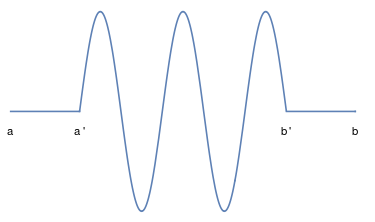
\includegraphics[scale=0.4]{./img/testfuncion.png}
\end{center}

Definimos $\Psi(x)=\integral{a'}{x}{\phi(s)ds}$ y tenemos $\Psi'=\phi$.

\end{proof}

\begin{lemma}
\label{lemma:14}
Sea $f\in C(a,b)$ tal que $\integral{}{}{f\phi'(x)dx=0}\espacio\forall\phi\in\mathcal{D}(a,b)\Longrightarrow f \text{ es constante.}$
\end{lemma}

\begin{proof}
Sea $x_0\in(a,b)$, por el lema \ref{existanciaphi}, podemos tomar $\phi_{x_0}\in \soportecompacto$, de forma que $\integral{a}{b}{\phi_{x_0}(s)ds}=1$ (multiplicándola por cierta constante). 

Definimos $\Psi(x)=\integral{a}{x}{\phi_{x_0}(s)ds}$ y tomamos $c$ de forma que:

\[
\integral{a}{b}{f(s)\Psi'(s)}=c\integral{a}{b}{\Psi'(s)ds}=c\Psi\Big|_a^b=c
\]

Tomamos $\phi\in\soportecompacto$ y veamos que la función $\phi-\lambda\Psi'$ tiene primitiva para cierto $\lambda\in\R$. Supongamos que tiene media 0, y despejemos $\lambda$:

\[
\integral{a}{b}{\phi(s)-\lambda\Psi'(s)}=0 \Longrightarrow \lambda=\integral{a}{b}{\phi(s)ds}
\]

Haciéndo esa elección de $\lambda$, $\phi-\lambda\Psi'$ tiene primitiva por el lema \ref{lemma:13}.

\[
0=\integral{a}{b}{f(s)(\phi(s)-\lambda\Psi'(s))ds}=\integral{a}{b}{f(s)\phi(s)ds}-\lambda\integral{a}{b}{f(s)\Psi'(s)ds}=
\]
\[
=\integral{a}{b}{f(s)\phi(s)ds}-c\integral{a}{b}{\phi(s)ds}=\integral{a}{b}{(f(s)-c)\phi(s)ds} \Rightarrow f(s)-c=0 \Rightarrow f\equiv 0
\]

\end{proof}

\begin{lemma}
Sean $f$,$g$ funciones continuas en $(a,b)$, entonces es equivalente:

\[
\integral{a}{b}{g\phi}+\integral{a}{b}{f\phi'}=0 \espacio \forall\phi\in\soportecompacto \Longleftrightarrow f\in C^1(a,b), g=f'
\]

\end{lemma}

\begin{proof}

($\Rightarrow$)Tomamos $x_0\in(a,b)$ y definimos $\tilde{f}(x)=\integral{a}{x}{g(s)ds}\Rightarrow \tilde{f}\in C^1$.

\[
\integral{a}{b}{\tilde{f}(s)\phi'(s)+g(s)\phi(s)ds}=\integral{a}{b}{\tilde{f}(s)\phi'(s)+\tilde{f}'(s)\phi(s)ds}=\integral{a}{b}{(\tilde{f}\phi)}=\tilde{f}\phi\Big|_a^b=0
\]

Restando la expresión de la hipótesis menos la anterior, obtenemos:

\[
0=\integral{a}{b}{f(s)\phi'(s)ds}-\integral{a}{b}{\tilde{f}(s)\phi'(s)ds}=\integral{a}{b}{(f-\tilde{f})(s)\phi'(s)ds}
\]

Y usnado el lema \ref{lemma:14}, tenemos que $f-\tilde{f}$ es constante, luego $f\in C^1$ ya que $\tilde{f}$ también pertenece a $C^1$.

($\Leftarrow$) 
\[
0=f\phi(x)\Big|_a^b=\integral{a}{b}{(f(x)\phi(x))'dx}=\integral{a}{b}{f(x)\phi'(x)dx+f'(x)\phi(x)dx}
\]

\end{proof}

\subsection{Ejemplos}

A continuación veremos un ejemplo teórico y algunos ejemplos más prácticos de la teoría anterior.

\subsubsection{Problema de Braquistocrona}

Este problema se centra principalmente en averiguar que forma (curva) tenemos que darle a un tobogán para que este sea el más rápido.

A esa curva la vamos a denotar por $Y(t)$ y vamos a suponer que  pertenece a $C^1(0,L)$, es decir, que no tenga picos. Además, vamos a suponer que el tobogán tiene altura máximo 1, y mínima 0, es decir, $Y(0)=1$ e $Y(L)=0$. También necesitamos que el tobogán tenga sentido, es decir, que no tenga subidas ni bajadas muy bruscas, luego necesitamos imponer $Y'(x)<1 \espacio \forall x \in (0,L)$.

Recordemos primero algunas nociones de física. Vamos a denotar por $(x(t),y(t))$ a la posición de una persona en el tobogán en el instante $t\in[0,L]$, por $m$ a su masa y por $g$ a la gravedad. Recordemos que la expresión de la energía es $mgy(t)$, la de la velocidad es $v(t)=\sqrt{x'(t)^2+y'(t)^2}$ y la de la energía cinética es $\frac{mv(t)^2}{2}$.

Si hacemos el tobogán suficientemente suave, se tiene que verificar lo siguiente:

\begin{equation}
\label{equationff}
mgy(t)+\frac{m}{2}(x'(t)^2+y'(t)^2)\equiv cte
\end{equation}
En el primer momento nos dejamos caer, luego en $t=0$, $(\ref{equationff})=mg$

Tenemos entonces $y(t)=Y(x(t)) \Rightarrow y'(t)=Y'(x(t))x'(t)$, sustituyendo en (\ref{equationff}):
\[
mgY(x(t))+\frac{m}{2}x'(t)^2+\frac{m}{2}(Y'(x(t))x'(t))^2=mg
\]
\[
x'(t)^2\left(1+Y'(x(t))^2\right)=2g\left(1-Y(x(t))\right)\Rightarrow x'(t)=\sqrt{2g}\sqrt{\frac{1-Y(x(t))}{1+Y'(x(t))^2}}
\]

Estamos buscando el tiempo de llegada, $T$, ¿cómo lo hacemos? Aplicamos un truco típico de ecuaciones diferenciales:

\[
T = \integral{0}{T}{dt}=\integral{0}{T}{\frac{x'(t)}{x'(t)}dt}=
\frac{1}{\sqrt{2g}}\integral{0}{T}{\frac{\sqrt{1+Y'(x(t))^2}}{\sqrt{1-Y(x(t))}}x'(t)dt}
\]

Que tras el cambio de variable $x=x(t)$ nos queda:

\[
T=\frac{1}{\sqrt{2g}}\integral{0}{L}{\frac{\sqrt{1+Y'(x)^2}}{\sqrt{1-Y(x)}}dx}
\]

Definimos ahora el conjunto de funciones donde vamos a buscar nuestro mínimo:
\[
D=\{y\in C^1(0,L),y(0)=1,y(L)=0, y'(x)<1 \espacio \forall x \in(0,L)\}
\]

Y definimos nuestro funcional:

\[
L_y=\integral{0}{L}{\frac{\sqrt{1+Y'(x)^2}}{\sqrt{1-Y(x)}}dx}
\]

Usando la notación del principio, tenemos una función $F$ tal que $F(x,y,p)=\sqrt{\frac{1+p^2}{1-y}}$

Usando el Teorema \ref{theorem:12} podemos definir:

\[
Z(x)=\derivada{F}{p}(x,y,y')=\frac{1}{\sqrt{1-y(x)}}\frac{y'(x)}{\sqrt{1+y'(x)^2}} \in C^1(0,T)
\]

Ahora, en lugar de despejar $y'(x)$, vamos a ver que $y\in C^2$. Definiendo $\Psi(y')=\frac{y'}{\sqrt{1+y'^2}}=Z(x)\sqrt{1+y'^2}$. Como $\Psi(s)=\frac{s}{\sqrt{1+s^2}}$ tiene inversa de clase 1, tenemos:

\[
y'(x)=\Psi^{-1}(Z(x)\sqrt{1-y(x)})\Rightarrow y\in C^2
\]

En general, tenemos que si $F$ no depende de $x$, podemos hacer:
\[D(x)=F(y,y')-Z(x)y'\Rightarrow D'(x)=\derivada{F}{y}(y,y')y'+\derivada{F}{p}(y,y')y''-Z'(x)y'-Z(x)y''=\]
\[
=y'(Z'(x)-Z'(x))=0
\]

Es decir, para alguna constante $C\in\R$, tenemos que:
\[
F(y,y')-Z(x)y'=C
\]

En nuestro caso particular, nos quedaría:

\[
\frac{\sqrt{1+y'(x)^2}}{1-y(x)}-\frac{1}{\sqrt{1-y(x)}}\frac{y'(x)^2}{\sqrt{1+y'(x)^2}}=0 \Rightarrow \frac{1}{\sqrt{1-y(x)}}\frac{1}{\sqrt{1+y'(x)^2}}=C
\]

Esa ecuación diferencial, es de variables separadas, deberíamos resolverla con las condiciones iniciales $y(0)=1,y(L)=0$, pero la solución es trascendente, es decir, no tiene expresión explícita, es un cicloide.

\begin{figure}[h!]
   \center
  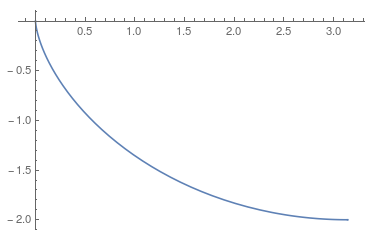
\includegraphics[scale=0.5]{img/cicloide.png}
  \caption{Ejemplo de cicloide}
\end{figure}

\subsubsection{Ejercicios prácticos}

\begin{ejercicio*}
Encontrar la curva en la que el siguiente funcional podría alcanzar su extremo:
\[
I(y)=\integral{1}{2}{\Big(y'(x)^2-2xy(x)\Big)dx}
\]

con condiciones de contorno $y(1)=0,y(2)=-1$.
\end{ejercicio*}

\textbf{Solucion:}

Definimos $F(x,y,p)=p^2-2xy$ y obtenemos:
\[
\derivada{F}{p}=2p, \espacio \derivada{F}{y}=-2x \Rightarrow Z(x)=2y'(x), \espacio Z'(x)=-2x
\]
Resolviendo la ultima ecuación, obteniendo:
\[
Z(x)=-x^2+C \Rightarrow 2y'(x)=-x^2+C \Rightarrow y'(x)=\frac{-x^2+C}{2}\Rightarrow y(x)=-\frac{x^3}{6}+\frac{c}{2}x+D
\]

Usando las condiciones de contorno, podemos calcular el valor de $C$ y $D$, obteniendo:

\[
y(x)=\frac{x-x^3}{6}
\]

\begin{ejercicio*}
Encuentra las curvas que unen $(1,3)$ con $(2,5)$, que puedan ser extremos del funcional:

\[
I(y)=\integral{1}{2}{\Big(y'(x)+x^2y'(x)^2\Big)dx}
\]
\end{ejercicio*}

\textbf{Solución} $y(x)=-\frac{4}{x}+7$

\subsection{Relación de ejercicios}

\begin{ejercicio}
Dado el funcional 
\[
\mathcal{F}(y(x))=\integral{a}{b}{\Phi(x,y(x),y'(x))dx}
\]

demuéstrese la equivalencia de las dos formas siguientes de Euler-Lagrange.

\[
\derivada{\Phi}{y}-\frac{d}{dx}\derivada{\Phi}{y'}=0 \espacio\espacio \derivada{\Phi}{x}-\frac{d}{dx}\left(\Phi-y'\derivada{\Phi}{y'}\right)=0
\]
\end{ejercicio}

\begin{ejercicio}
Obténgase la forma que adopta la ecuación de Euler-Lagrange en los siguientes casos particulares:

\begin{enumerate}[a)]
\item $\Phi$ sólo depende de $y'$.
\item $\Phi$ no depende de $y$.
\item $\Phi$ no depende explícitamente de $x$.
\item $\Phi=G(x,y)\sqrt{1+y'^2}$.
\end{enumerate}
\end{ejercicio}

\begin{ejercicio}
Aplíquense los resultados anteriores a los ejemplos siguientes:
\begin{enumerate}[a)]
\item $\mathcal{F}(y(x))=\integral{}{}{y(2x-y)dx}$, $y(0)=0$, $y(\pi/2)=\pi/2$.
\item $\mathcal{F}(y(x))=\integral{}{}{(y^2+2xyy')dx}$, $y(a)=A$, $y(b)=B$.
\item $\mathcal{F}(y(x))=\integral{}{}{y'(1+x^2y')dx}$, $y(1)=3$, $y(2)=5$.

\end{enumerate}
\end{ejercicio}

